% sections/prefetching.tex
% TJ WILL WRITE THIS SECTION !!!

This section explains the concept of link prefetching and discusses a possible usage of it as a defense mechanism against fingerprinting attacks on Tor.

\subsection{Link Prefetching}

% introduction about link prefetching
Link prefetching is a HTML syntax that gives the web browser hints about which page the user is most likely to visit in a near future~\cite{fisher2003, fisher2004link}. 
The pages and resource to pre-fetch are specified in the web page so that the web browser can silently load them (or pre-fetch them) after an idle time.
Since the pre-fetch happens only after the page is fully loaded, it does not sacrifice the loading time of the requested web page.
Moreover, it can save the loading time for the pre-fetched pages and thus improve the user experience by caching the {\it future} contents.
It was first suggested by Mozilla Foundation in 2003 and supported by most modern browsers nowadays.

\iffalse %commented out
Once the web contents provider is reasonably certain about which links the users are most likely to visit next, it can improve the user experience by saving the loading time. 
Particularly, it is most effective if the content provider may be reasonably certain which links users are going to visit next.
Having been first suggested by Mozilla Foundation, it is adopted by most modern browsers nowadays.
Today's web browsers makes use of a specific syntax called \emph{pre-fetching}, which was proposed as a draft standard by Mozilla.
Using pre-fetching, browser can predicts documents likely to be visited by the user in the near future.
Therefore, based on the hint provided by pre-fetching a browser is able to fetch those documents a head of time.
In fact, it is the web page that provides a set of pre-fetching hints for the browser.
Then, loading the page and passing an idle time, the browser starts to pre-fetch and cache specified documents.
Needless to say, this mechanism improves efficiency.
\fi
% Insert a figure of "prefetch-network" which shows the network traffic.
% explain about how prefetching actually works 

The resources to prefetch can be simply specified in {\it HTML} using a {\tt link} tag~\cite{nottingham2010}.
For example, a {\tt link} tag {\tt <link rel="p\-refetch" href="/page2.html">} tells the browser to pre-fetch a {\it html} file named {\it page2.html}.
Resources other than a {\it HTML} web page can also be pre-fetched similarly using the same syntax.
There are also some variations for different types of prefetching -- DNS prefetching, which is specified as {\tt <link rel="dns-prefetch" ..>}, is supported by {\it Mozilla Firefox} and {\it Google Chrome}, and {\tt <link rel="prerender" ..>} also does the same job as {\tt prefetch} in {\it Google Chrome} and {\it Microsoft Internet Explorer}.

Figure~\ref{fig:network} illustrates how prefetching actually works in a browser ({\it Google Chrome}).
This page is set up arbitrarily by the authors to demonstrate link prefetching, and contains a link pre-fetch tag that specifies to load a big image (the image on the left side labeled as {\it prefetch}).
When the prefetching is off, this image shall be requested only when a user puts his mouse cursor on it (mouse over).
However, it can be seen on the network timeline (right bottom) that the image is pre-fetched right after loading the page.
This is indicated by a long blue bar on the second row for the file named {\it Very-high...}, and it is long because the size of the file is relatively big ({\it 3.5 MB}) that it took a relatively long time to download.
Please also note that the time it took for loading the image when the user actually requested (by putting his mouse on it) was very short, because the image had already been pre-fetched that the browser merely loaded it from the cache (as shown in the {\it size} column on the fourth row).

\begin{figure*}[h]
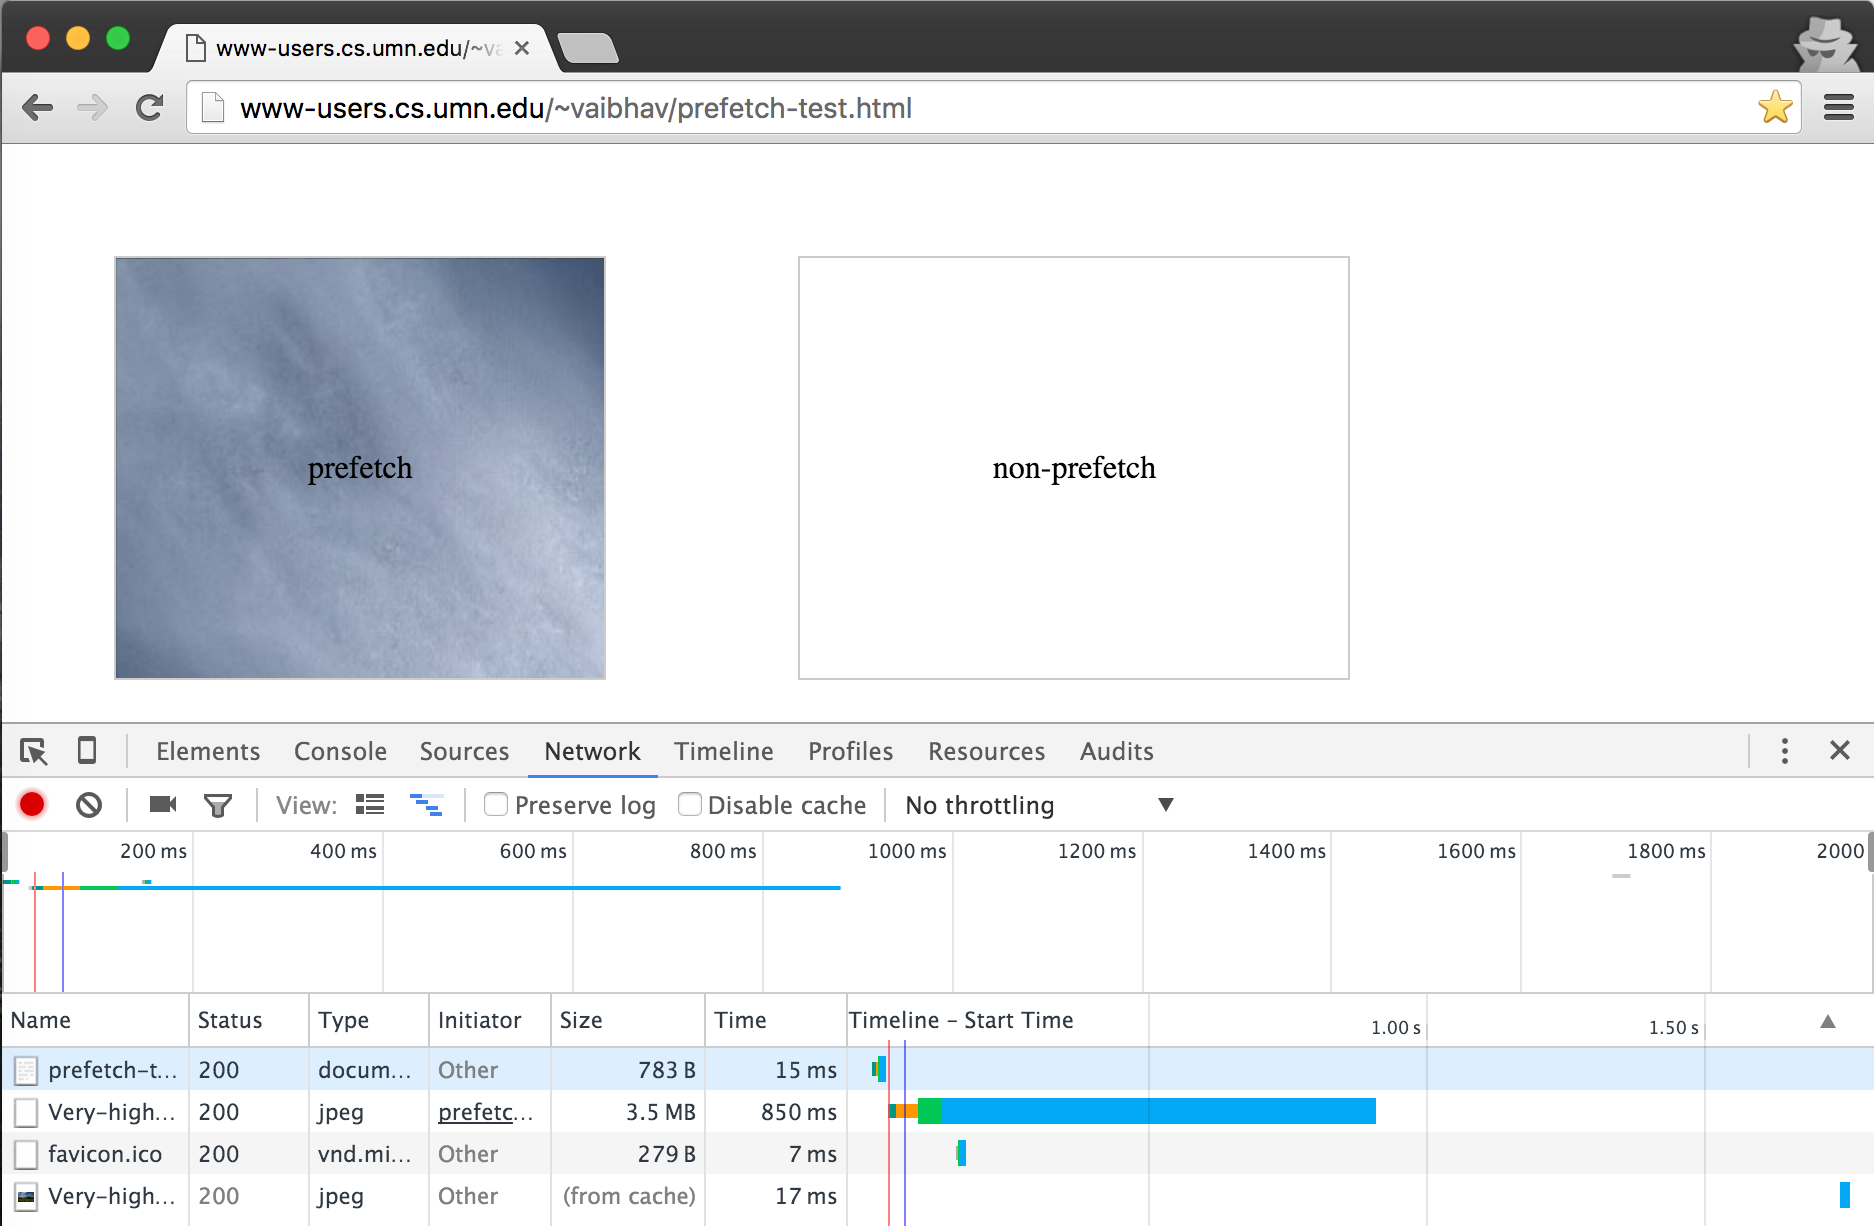
\includegraphics[width=\textwidth]{figures/prefetch-network.png}
\centering
\caption{Network timeline showing pre-fetch}
\label{fig:network}
\end{figure*}

\subsection{The Effect of Prefetching on Fingerprinting}
% cite some papers to describe about the features that are used for attacks,
% and explain why prefetching change the feature.
% Vaibhav says: put the intuition down 

The idea of studying the effect of prefetching on Tor network is not new~\cite{something}.

Figure~\ref{fig:prefetch} shows an aspect of fingerprint we gathered for the firt page of {\tt www.wired.com}.
It depicts the number of packets on the {\it y-axis} for each time interval ({\it 500 ms}), where the {\it x-axis} represents the time in seconds.
The solid line represents the number of packets throughout time when the pre-fetch feature was enabled, and the dashed line represents when the pre-fetch was disabled in the browser settings.

\begin{figure}[h]
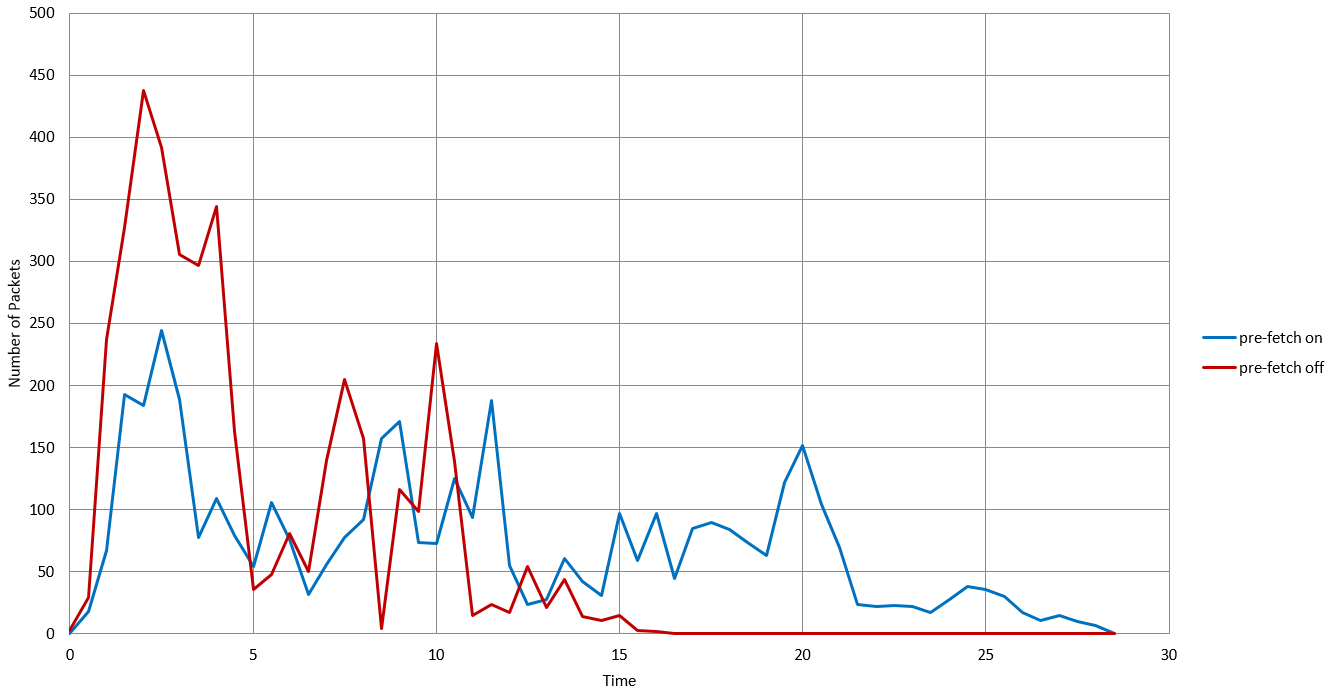
\includegraphics[width=\columnwidth]{figures/prefetch.png}
\centering
\caption{hi}
\label{fig:prefetch}
\end{figure}


